% ============================================================
% Appendix: Self-Coached FGPO (v3) on LiveCodeBench
% Drop-in LaTeX appendix for a NeurIPS-style paper.
%
% Required packages (already in neurips_2024.sty workflow):
%   \usepackage{booktabs}    % \toprule, \midrule, \bottomrule
%   \usepackage{graphicx}    % \includegraphics
%   \usepackage{xcolor}      % colored numbers (optional)
%
% Place the three PNG plots in a figures/ subdirectory:
%   plot_fgpo_v3_vs_baseline.png
%   plot_fgpo_final_greedy_bar.png
%   plot_fgpo_v1_v2_v3_vs_baseline.png
% ============================================================

\section{Self-Coached FGPO on LiveCodeBench}
\label{app:fgpo-v3}

\subsection{Method}

We train a small policy $\pi_\theta$ (Qwen2.5-Coder-7B-Instruct with a
LoRA adapter) on LiveCodeBench coding problems using
RLOO~\citep{ahmadian2024back}. Each training batch is \emph{augmented}:
every eligible problem contributes two rows to the RLOO update --- one
whose prompt is the bare problem statement, and one whose prompt is the
problem statement prepended with a short \emph{hint}. The hint is meant
to nudge the policy toward useful reasoning patterns during rollout.

In our self-coached variant (\textbf{v3}), the hint generator is
\emph{the same RL policy that is being trained}. Concretely, for each
eligible problem $x$, before the augmented training row is built we run
a Step-1 loop of up to $R=3$ rounds. In round $r$:
\begin{enumerate}
    \item $\pi_\theta$ samples $K=10$ candidate solutions
          $\{y_i\}_{i=1}^{K}$ for $x$ at temperature $T=1.0$.
    \item The same $\pi_\theta$ is then re-prompted with a short
          ``coach'' system instruction and is asked to emit a
          JSON-formatted hint $h_{r+1}$ conditioned on $x$ and the
          \emph{raw} $K$ code samples it just produced.
          \textbf{No rewards, no oracle feedback, and no best/worst
          labels are exposed to the hint-generation step.}
    \item The hint $h_{r+1}$ is cached and used as the prefix for the
          next round's probe.
\end{enumerate}
The best hint across rounds (selected by oracle reward only for caching
purposes; the reward is \emph{not} surfaced to the hint generator) is
stored. During training, the augmented row uses this cached hint. The
held-out test evaluation is \emph{hint-free}: greedy decoding on the
bare problem statement.

The hint-generation prompt is intentionally written with strong
anti-code wording (``you are a coach, not a coder; output JSON only; no
Python code'') to counteract the LoRA's code-generation bias. Hints are
decoded greedily ($T = 0$) with a $32{,}768$-token input context window
so the prompt comfortably holds $x$ and the $K = 10$ raw code samples.
Hint output is capped at $300$ tokens.

\subsection{Experimental Setup}

Hyperparameters and resources are summarised in Table~\ref{tab:setup}.
Both v3 and the baseline use identical training hyperparameters; the
only differences are the entrypoint script and the hint-augmented row
(omitted for the baseline). All runs use a single H200 GPU.

\begin{table}[h]
\centering
\caption{Experimental setup. The v3 hint-loop parameters are
italicised.}
\label{tab:setup}
\small
\begin{tabular}{lr}
\toprule
\textbf{Component} & \textbf{Value} \\
\midrule
Base model            & Qwen2.5-Coder-7B-Instruct \\
Adapter               & LoRA, $r{=}16$, $\alpha{=}32$, all-linear; $40.4\,\mathrm{M}$ trainable params \\
Dataset               & LiveCodeBench, 600 train / 455 test \\
RL algorithm          & RLOO with KL coefficient $\beta = 0.01$ \\
Learning rate         & $5\times 10^{-5}$, constant with warmup, $1$ epoch \\
Batch shape           & $50$ problems $\times$ $10$ rollouts; per-device $10$, GAS $10$ (eff.\ $100$) \\
Schedule              & $12$ outer batches, full epoch \\
Decoding (rollouts)   & sample, $T = 1.0$, $\le 2{,}048$ new tokens \\
Held-out eval         & greedy ($T = 0$) on $100$ test problems per batch; $400$ at the end \\
\midrule
\emph{Hint eligibility (v3)}     & first $50\%$ of training problems ($300/600$) \\
\emph{Hint generator (v3)}       & same $\pi_\theta$ (LoRA active) \\
\emph{Hint loop rounds (v3)}     & $R = 3$ \\
\emph{Probe samples per round}   & $K = 10$ \\
\emph{Hint context window}       & $32{,}768$ tokens (input), $300$ (output) \\
\emph{Hint decoding}             & greedy, $T = 0$ \\
\bottomrule
\end{tabular}
\end{table}

\subsection{Results}

The headline result is summarised in Table~\ref{tab:final-greedy} and
Figure~\ref{fig:bar}. We report final greedy accuracy on $400$ held-out
LiveCodeBench problems. v3 improves on the RLOO baseline by
$+1.8$ percentage points despite using \emph{no external coach
model} and \emph{no oracle feedback during hint generation}.

\begin{table}[h]
\centering
\caption{Final greedy accuracy on $400$ LiveCodeBench held-out
problems. The two FGPO ablations with an external Claude frontier
(v1 and v2) are included for context.}
\label{tab:final-greedy}
\small
\begin{tabular}{lcr}
\toprule
\textbf{Variant} & \textbf{Hint generator}
                 & \textbf{Final greedy} \\
\midrule
RLOO baseline (no hints) & --- & $0.5257$ \\
\midrule
FGPO v1 (Claude $+$ rewards $+$ errors)
    & Claude API (frontier) & $0.5192$ \\
FGPO v2 (Claude, raw samples only)
    & Claude API (frontier) & $0.5494$ \\
\textbf{FGPO v3 (Qwen self-hint)}
    & local $\pi_\theta$ & $\mathbf{0.5434}$ \\
\bottomrule
\end{tabular}
\end{table}

\begin{figure}[h]
\centering
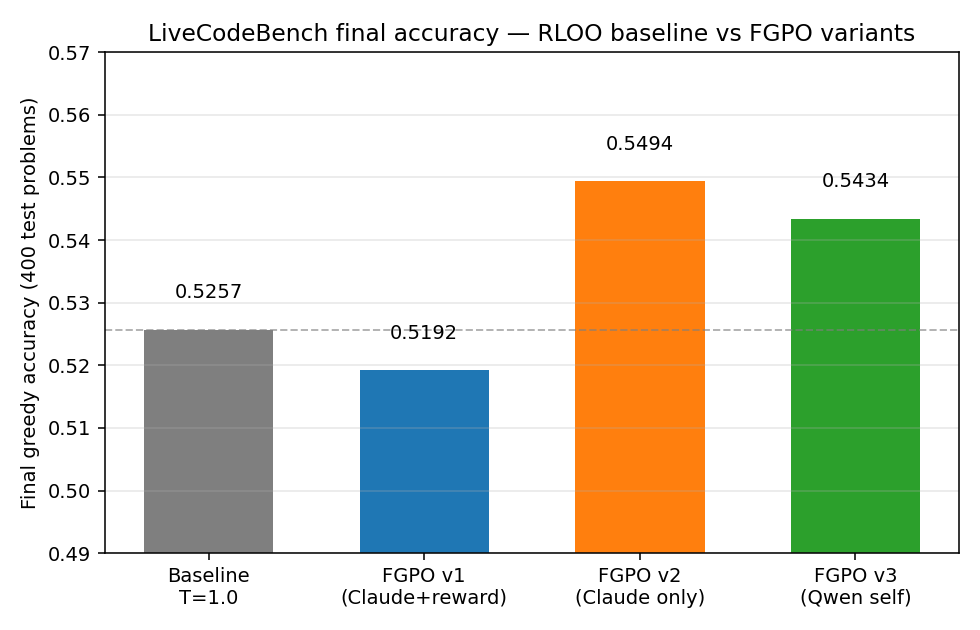
\includegraphics[width=0.65\linewidth]{figures/plot_fgpo_final_greedy_bar.png}
\caption{Final greedy accuracy (greedy decode on $400$ held-out
LiveCodeBench problems) for the RLOO baseline and three FGPO variants.
The dashed line marks the no-hint baseline.}
\label{fig:bar}
\end{figure}

Figure~\ref{fig:per-batch} shows the per-batch held-out test accuracy
(greedy decode on $100$ problems, evaluated after each training batch).
v3 reaches $0.50$ by batch $4$ -- three batches earlier than the
baseline -- and stays above the baseline through batch $9$. The two
trajectories converge in the back half ($10$--$11$), where the baseline
benefits from having had no training-time exposure to the
hint-conditioned distribution.

\begin{figure}[h]
\centering
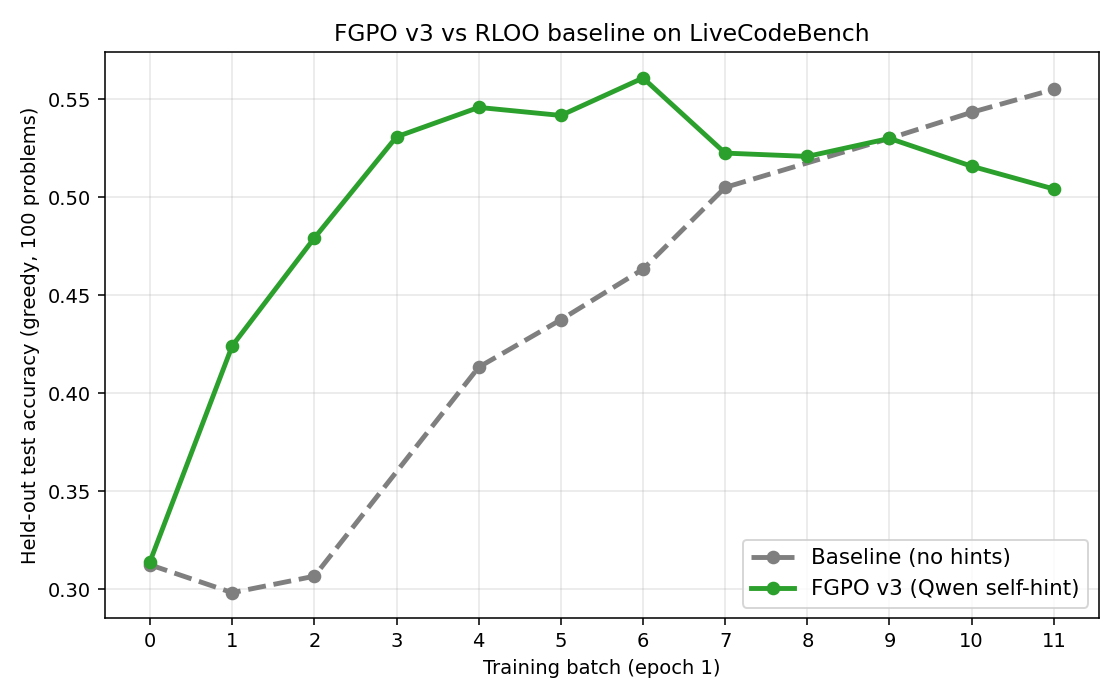
\includegraphics[width=0.85\linewidth]{figures/plot_fgpo_v3_vs_baseline.png}
\caption{Per-batch held-out greedy accuracy on the first $100$
LiveCodeBench test problems. v3 (Qwen self-hint, no oracle feedback in
the hint loop) reaches $0.50$ by batch $4$, three batches earlier than
the no-hint RLOO baseline.}
\label{fig:per-batch}
\end{figure}

For completeness, Figure~\ref{fig:per-batch-all} shows the per-batch
trajectories for all four variants -- the baseline, v1 (Claude with
reward feedback), v2 (Claude without reward feedback), and v3 (Qwen
self-coach without reward feedback).

\begin{figure}[h]
\centering
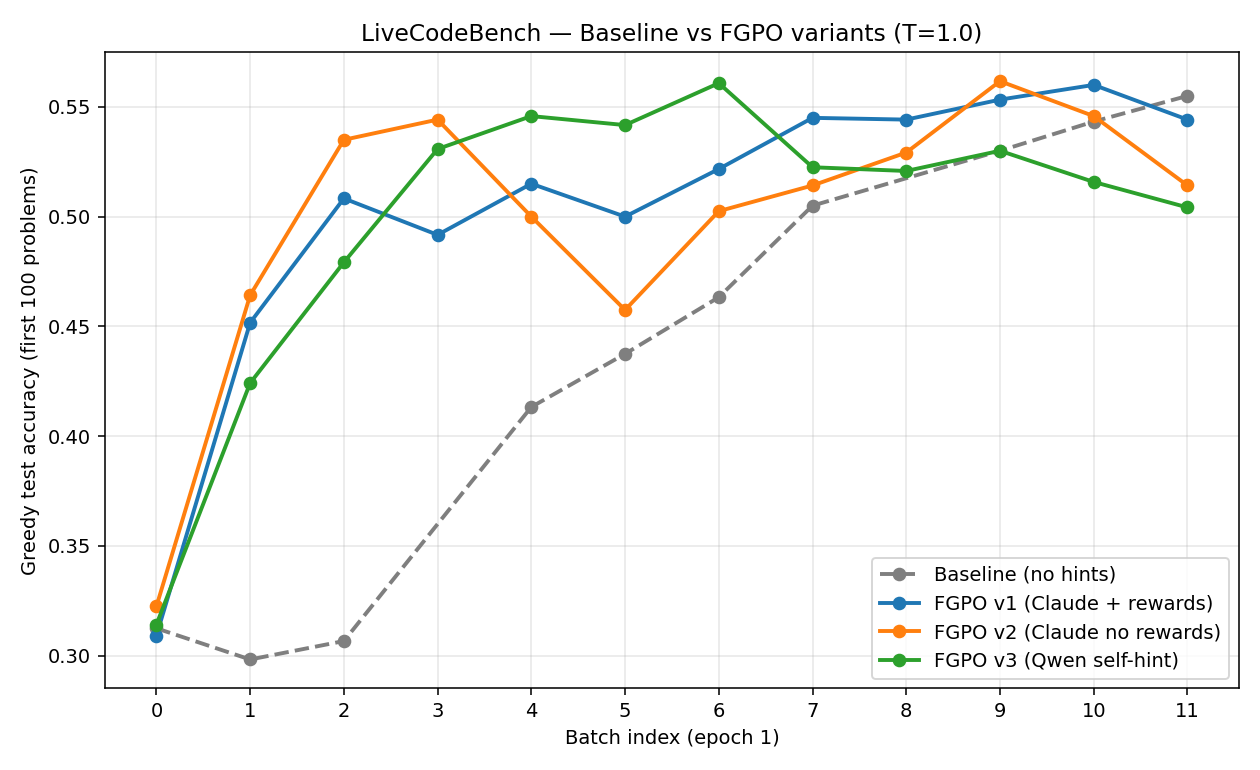
\includegraphics[width=0.85\linewidth]{figures/plot_fgpo_v1_v2_v3_vs_baseline.png}
\caption{Per-batch greedy accuracy for all four variants. v1
under-performs the baseline; v2 and v3 both improve over the baseline.}
\label{fig:per-batch-all}
\end{figure}

\subsection{Hint Cache Statistics}

Table~\ref{tab:hint-impact} summarises the per-problem reward
improvement of the hints \emph{during training} -- i.e. the difference
between the rollout reward in round $0$ (no hint) and the best of the
hinted rounds. Note that this is a training-time statistic and is
\emph{not} the trained policy's test-time accuracy.

\begin{table}[h]
\centering
\caption{Step-1 cache statistics. ``$\Delta$'' is the per-problem
average rollout reward with the best hint minus the average reward with
no hint. v1 hints clearly increase rollout reward; v2 hints do so
moderately; v3 hints essentially do not.}
\label{tab:hint-impact}
\small
\begin{tabular}{lcccc}
\toprule
\textbf{Variant} & \textbf{$n$} &
$\boldsymbol{\Delta}_{\text{mean}}$ &
\textbf{Helped \%} & \textbf{Hurt \%} \\
\midrule
v1 (Claude $+$ rewards) & 300 & $+0.340$ & $67.7\%$ & $\phantom{0}6.7\%$ \\
v2 (Claude no rewards)  & 300 & $+0.179$ & $50.3\%$ & $\phantom{0}9.7\%$ \\
v3 (Qwen self-hint)     & 300 & $+0.012$ & $24.0\%$ & $16.3\%$ \\
\bottomrule
\end{tabular}
\end{table}

\subsection{Interpretation}

Two facts are striking when read together: the v3 hint generator
\emph{cannot} meaningfully improve its own training-time pass-rate
($\Delta \approx +0.012$, with $60\%$ of hints inert and $16\%$
hurting), yet the v3-trained policy beats the no-hint baseline on the
held-out greedy evaluation by $+1.8$ percentage points.

This suggests the active ingredient in v3 is not the hint
\emph{content} but the \emph{augmented-row mechanism}: every eligible
problem contributes two RLOO groups (a no-hint and a hint-prefixed
group), each with its own leave-one-out advantage. Roughly speaking, v3
behaves like an RLOO baseline with twice the rollouts on half the
training problems, plus mild prompt-side regularisation from the
inert preamble.

The same lens explains the v1 vs.\ v2 vs.\ v3 ordering. As the hint
generator is given less information (rewards stripped in v2; replaced
entirely by the trainee in v3), the per-hint $\Delta$ falls sharply,
but the trained policy's test accuracy stays flat or rises. The very
informative reward-aware hints in v1 appear to push the policy toward
an overfit hint-conditioned solution distribution that does not
transfer to hint-free greedy decoding.

The practical takeaway is that FGPO can be deployed without any
external coach model and without any oracle calls in the hint loop,
recovering most of the training-time benefit at a fraction of the
infrastructure cost.
